\section{SeismicSpider}\label{sec:SeismicSpider}
\begin{figure} \centering
  {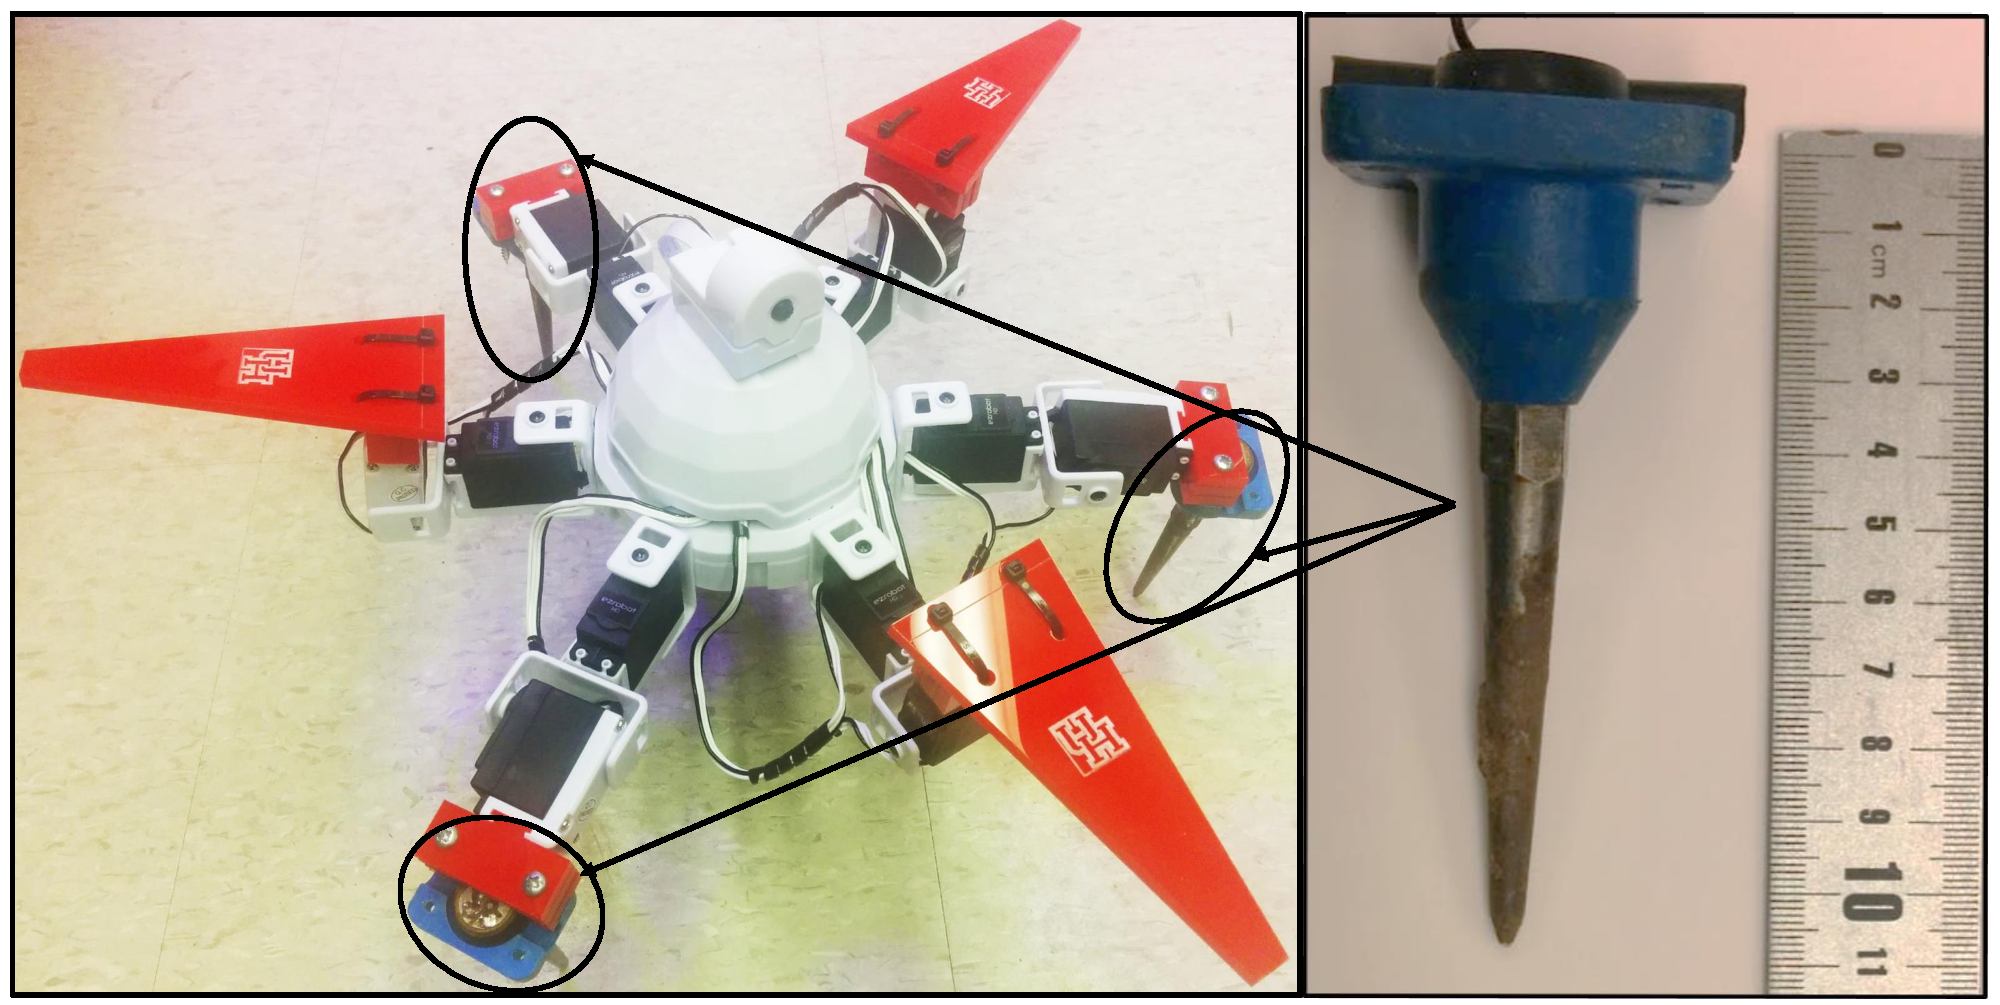
\includegraphics[width=\columnwidth]{Hex_overview.pdf}}
 \caption{The hexapod sensor is a mobile unit with three of it's legs replaced by geophones. It has the ability to sense seismic waves and store the data obtained.} 
 \label{fig:TradvsAutoDrop}
\end{figure}
\subsection{Design}

\subsection{Experiments}
\subsubsection{Exp 1: Accuracy plot}
Hexapod move to desired GPS location  (plot accuracy)\\
\subsubsection{Exp 2: Shot gather comparison}
Hexapod sensing accuracy vs ground setup\\
\begin{figure} \centering
  {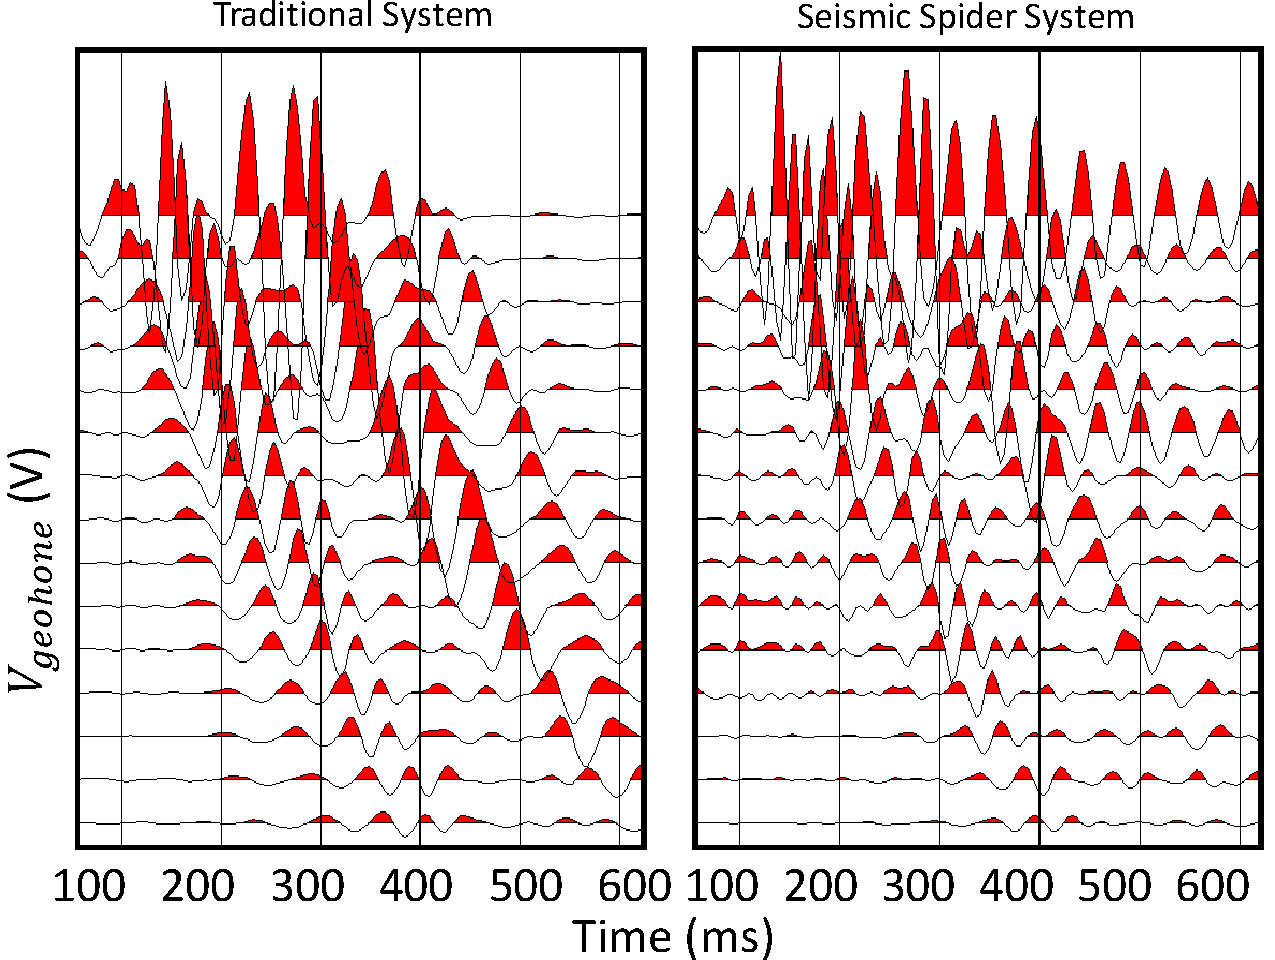
\includegraphics[width=\columnwidth]{shotgather_hex.pdf}}
 \caption{Shot gather comparison of traditional geophones vs hexapod sensor a.) Traditional b.) Hexapod} 
 \label{fig:TradvsAutoDrop}
\end{figure}
\subsubsection{Exp 3: Deploying and Retrieving Hexapod}
Exp 5: Retrieving Hexapod\\